\documentclass[8pt, aspectratio=169]{beamer}
\usetheme{Frankfurt}
\usecolortheme{beaver}

\usepackage[spanish]{babel}
\usepackage{amsmath}
\usepackage{amsfonts}
\usepackage{amssymb}
\usepackage{color}
\usepackage{xcolor}
\usepackage{listings}
\usepackage{graphicx}
\usepackage{wrapfig}

\definecolor{codegreen}{rgb}{0,0.6,0}
\definecolor{codegray}{rgb}{0.5,0.5,0.5}
\definecolor{codepurple}{rgb}{0.58,0,0.82}
\definecolor{backcolour}{rgb}{0.95,0.95,0.92}

\lstdefinestyle{mystyle}{
    commentstyle=\color{codegreen},
    keywordstyle=\color{magenta},
    numberstyle=\tiny\color{codegray},
    stringstyle=\color{codepurple},
    basicstyle=\ttfamily\footnotesize,
    breakatwhitespace=false,         
    breaklines=true,                 
    captionpos=b,                    
    keepspaces=true,                 
    numbers=left,                    
    numbersep=5pt,                  
    showspaces=false,                
    showstringspaces=false,
    showtabs=false,                  
    tabsize=2,
	xleftmargin=8pt
}

\lstset{style=mystyle, basicstyle=\scriptsize}

\author{Shao Jie Hu Chen \and Mario Megías Mateo \and Jesús Samuel García Carballo}
\title{Práctica 1. Análisis de Eficiencia de Algoritmos}
\subtitle{Algorítmica}
%\logo{
\includegraphics[scale=0.05]{logo-ugr.jpeg}}
\institute{Universidad de Granada}
%\date{}
%\subject{}
%\setbeamercovered{transparent}
\setbeamertemplate{navigation symbols}{}

\begin{document}
	
	\begin{frame}[plain]
		\maketitle
		% \begin{center}
		% 	
\includegraphics[scale=0.15]{logo-ugr.jpeg}
		% \end{center}
	\end{frame}
	
	\begin{frame}
		\frametitle{Índice de contenidos}
		\tableofcontents
	\end{frame}

	\section{Introducción}

	\begin{frame}
		\frametitle{Objetivos}

            Los objetivos de esta práctica son los siguientes:
            \begin{itemize}
                \item \textbf{Estudio teórico, empírico e híbrido} y \textbf{comparación} de los algoritmos de ordenación más empleados, verificando los resultados teóricos.
                \item \textbf{Estudio teórico, empírico e híbrido} de algoritmos de alta complejidad, poniendo especial énfasis en su \textbf{viabilidad} en diferentes equipos. 
                \item Estudio del \textbf{aumento de eficiencia} de un mismo algoritmo para diferentes \textbf{tipos de optimización} del compilador. 
                \item Determinación del algoritmo \textbf{más adecuado} para cada situación en función del estado de los datos.
            \end{itemize}

	\end{frame}

	\begin{frame}

        \frametitle{Equipo}

        \begin{block}{ASUS}
			\begin{itemize}
				\item \textbf{Modelo}: ZenBook 15 UX534F
				\item \textbf{Procesador}: Intel(R) Core(TM) i7-10510U CPU @ 1.80GHz5
				\item \textbf{Memoria Ram}: 16 GB DDR4 @ 2.133 MHz.
				\item \textbf{Sistema Operativo} Ubuntu 20.04.2 LTS
			\end{itemize}
		\end{block}
            
        \begin{block}{HP}
            \begin{itemize}
				\item \textbf{Modelo}: Pavilion Gaming Laptop 15-dk0xxx
				\item \textbf{Procesador}: Intel(R) Core(TM) i7-9750H CPU @ 2.60GHz
				\item \textbf{Memoria RAM:} 32 GB DDR4
				\item \textbf{Sistema Operativo}: Ubuntu 20.04.4 LTS
			\end{itemize}
        \end{block}

        \begin{block}{LENOVO}
            \begin{itemize}
				\item \textbf{Modelo}: YOGA 530-14IKB
				\item \textbf{Procesador}: Intel(R) Core(TM) i5-8250U CPU @ 1.60GHz
				\item \textbf{Memoria RAM:} 8 GB DDR4
				\item \textbf{Sistema Operativo}: Ubuntu 20.04.4 LTS
			\end{itemize}
        \end{block}
    \end{frame}

    \begin{frame}
        \frametitle{GraphKiller}    
        \begin{figure}[H]
			\centering
			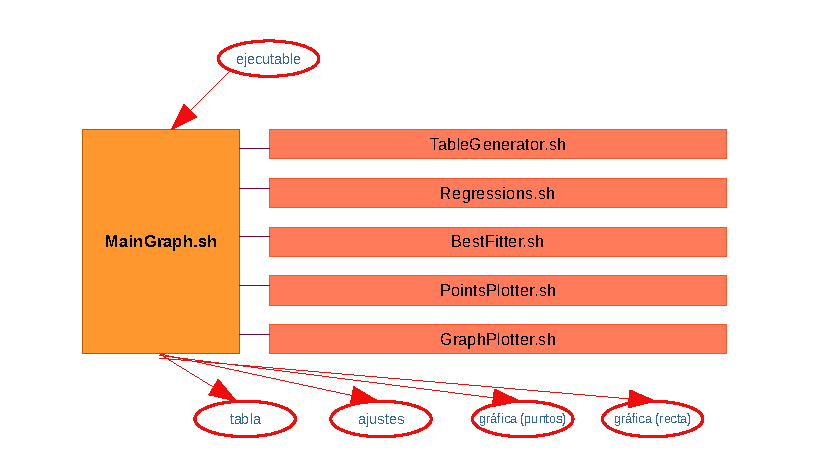
\includegraphics[width=0.67\textwidth]{img/esquema_graphkiller.pdf}
			\caption{Esquema del funcionamiento de GraphKiller}
			\label{graph-killer}
		\end{figure}
    \end{frame}

    \section{Eficiencia teórica}

    \begin{frame}[fragile]
        \frametitle{Algoritmo HeapSort}
   
        
        
        % \begin{itemize}
        %     \item \textbf{HeapSort}: $O(nlog(n))$
        %     \item  \textbf{QuickSort}: $T(n) \in O(nlog_{2}(n))$ si n $\geq$ UMBRAL.
        %     \item  \textbf{Inserción}: 
        %     \item  \textbf{Selección}:
        %     \item  \textbf{Heaport}:
        %     \item  \textbf{Heaport}:
        %     \item  \textbf{Heaport}:
        % \end{itemize}

        \begin{columns}
			% Column 1
			\begin{column}{0.5\textwidth}
				\begin{exampleblock}{Ejemplo de código}
                    \lstinputlisting[language=C++, firstline=56, lastline=68]{../src/heapsort.cpp} 
                \end{exampleblock}
			\end{column}
			% Column 2    
			\begin{column}{0.5\textwidth}

				\begin{exampleblock}{Ejemplo de código}
                    \lstinputlisting[language=C++, firstline=56, lastline=68]{../src/heapsort.cpp} 
                \end{exampleblock}

				

			\end{column}
			\end{columns}
    \end{frame}

    \section{Conclusiones}

    % \begin{frame}
    %     \frametitle{Conclusiones}
    %     Los aspectos tratados más relevantes son:
    %     \begin{itemize}
    %         \item \textby{Comprobar que los análisis empíricos verifican o no los resultados teóricos esperados}. Calculado los coeficientes de 
    %         determinación comprobamos que la función de regresión que mejor se ajusta en cada caso coincide con el tipo de función
    %         \item a
            
    %     \end{itemize}
        
    % \end{frame}

    \section{Eficiencia empírica}

    \begin{frame}
        \frametitle{Algoritmo de Inserción}

        
    \end{frame}

    \section{Referencias}

    \begin{frame}
        \begin{thebibliography}{0}
            \bibitem{Verdegay2017} Verdegay Galdeano. (2017). Lecciones de Algorítmica / José Luis Verdegay. Técnica Avicam.
            \bibitem{Cormen2017} Cormen. (2017). Introduction to algorithms / Thomas H. Cormen... [et al.] (3rd ed.). PHI Learning.
            \bibitem{Garrido2018} Garrido Carrillo. (2018). Estructuras de datos avanzadas: con soluciones en C++ / A. Garrido. Universidad de Granada.        
        \end{thebibliography}
    \end{frame}
    

	
\end{document}